\begin{figure*}
  \centering
  \begin{subfigure}[b]{\textwidth}
    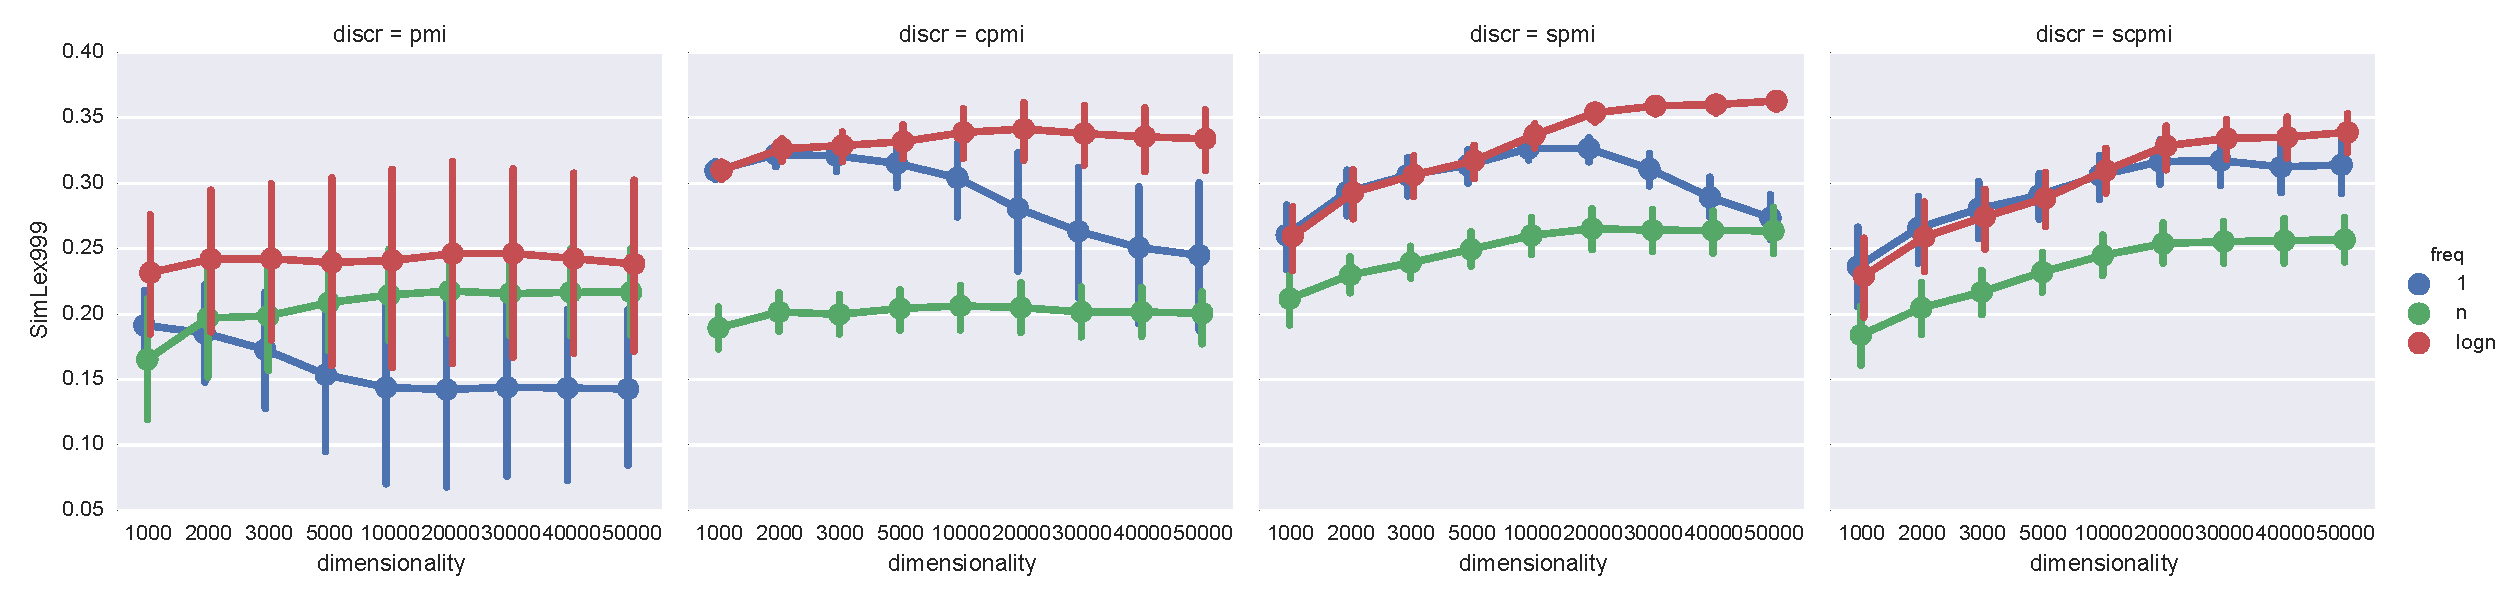
\includegraphics[width=\textwidth]{supplement/figures/SimLex999-performance-mean}
  \caption{Mean.}
  \label{fig:performance-mean}
  \end{subfigure}

  \begin{subfigure}[b]{\textwidth}
    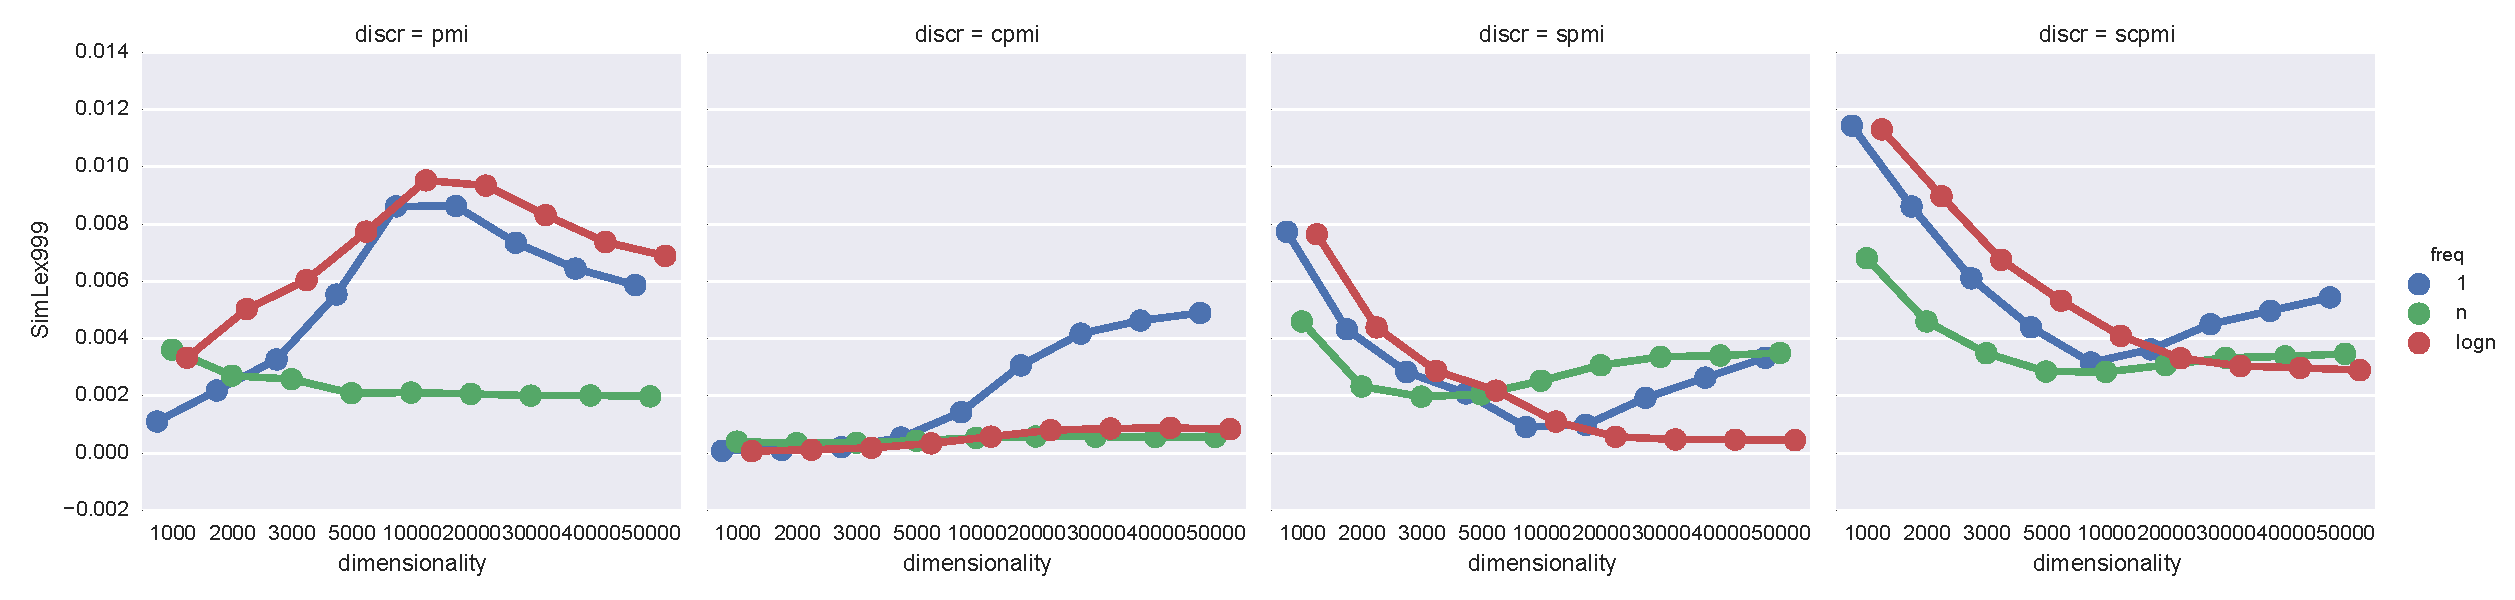
\includegraphics[width=\textwidth]{supplement/figures/SimLex999-performance-var}
  \caption{Variance.}
  \label{fig:performance-var}
  \end{subfigure}

  \caption{\textbf{Mean performance and variance.}}
  \label{fig:performance-mean-var}

\end{figure*}

%%% Local Variables:
%%% mode: latex
%%% TeX-master: "paper"
%%% End:
